\chapter{Software Parallelisability Metrics} \label{metrics}
\qquad This chapter defines proposed software source code parallelisability metrics and gives the basic intuition behind them. Proposed metrics inherited dependence-based nature from the work \cite{optimizing-compilers-book}. This book is built on and describes the results gathered through countless years of research and tremendous amount of work done in the field of optimizing compilers and high-performance computer architectures. \newline\null\qquad The chapter is structured in the following way. Section \ref{metrics-foundation-and-perspective} puts the metrics work into the context and gives the general perspective from which one has to look at parallelisability metrics. Section \ref{metrics-metric-groups} introduces the actual metrics, along with the basic motivation for them. Metrics are introduced as a set of conceptual groups. Each group has roughly the same intuition and motivation for all its metrics.  

\section{General foundation and perspective of the work} \label{metrics-foundation-and-perspective}

\subsection{Diversity in modern computer languages}
\label{metrics-diversity-in-modern-computer-languages}
\qquad There are thousands of different languages in the modern field of computer science. Computer programming languages have passed a long way from assembly languages operating at the level of native machine instructions to languages operating with concepts at a much higher abstraction levels. The reason behind such a change in the domain of computer languages is the ease, with which a human programmer can write a software. \newline
\null\qquad Unfortunately, this move to a higher-level languages comes with drawbacks as well. With the gain in programmer's productivity, such change also brings losses in software performance. It becomes increasingly difficult for the compiler to translate abstract languages into the sequence of machine instructions effectively. \newline
\null\qquad If we are to use these easy for human comprehension high-level languages, we must have tools for their efficient transformation into the form, suitable for direct execution on different native machine platforms.

\subsection{The modern role of compilers}
\label{metrics-modern-role-of-compilers}
\quad As was outlined in the previous section \ref{metrics-diversity-in-modern-computer-languages}, novadays compilers perform enabling role for the use of different sorts of modern computer languages. \newline
\null\quad In the modern state of the field, the principal role of compiler is to map high-level algorithms onto different sorts of high-performance architectures. The notion of high-performance architectures is really general and usually represents the combining term for all of the following: parallel cluster, multi-core and multi-processor architectures, vector processors, pipelined superscalar processors and all the possible combinations and co-designs of these. \newline
\null\quad Before this mapping can be done, compilers must perform extensive analyses to determine what parts of program computations depend on one another and what parts can be scheduled for parallel execution on high-performance machines. These analyses are mostly dependence-based by their nature.   

\subsection{The famous 80/20 rule}
\label{metrics-famous-80-20-rule}
\qquad Loops and arrays the most fertile ground for optimizations

\subsection{Dependence-based approach to metrics computation}
\label{metrics-dependence-based-approach}
\qquad Program parallelisation of program statements is basically hindered by the execution-order constraints imposed on those statements, which, in turn, are defined by different sorts of program dependencies, which were described in the section \ref{background-dependence-theory} of the thesis.   

\section{Metrics use}
\label{metrics-use}
\qquad Ideally, metrics should provide a quantitative measure of loop's algorithmic parallelisability (say, this loop is 80\% parallelisible). While existent modern tools (like \ref{background-modern-parallelisability-advisor-tools}) give answers only in binary format: yes, this loop has been parallelised or no, it hasn't been parallelised.

\section{Metric Groups}
\label{metrics-metric-groups}
\qquad The whole set of proposed metrics is divided into several concepual groups. To provide an illustrative description of different metrics, let's consider a loop \ref{lst:metrics-loop-example} given below. This loop is taken form EP NAS benchmark (see \ref{benchmarks}).
\begin{lstlisting}[caption={Example loop, taken from EP NAS benchmark}, captionpos=b, label=lst:metrics-loop-example]
for (i = 0; i < NQ; i++) {
	gc = gc + q[i];
}
\end{lstlisting}

\begin{figure}[htb]
	\centering
	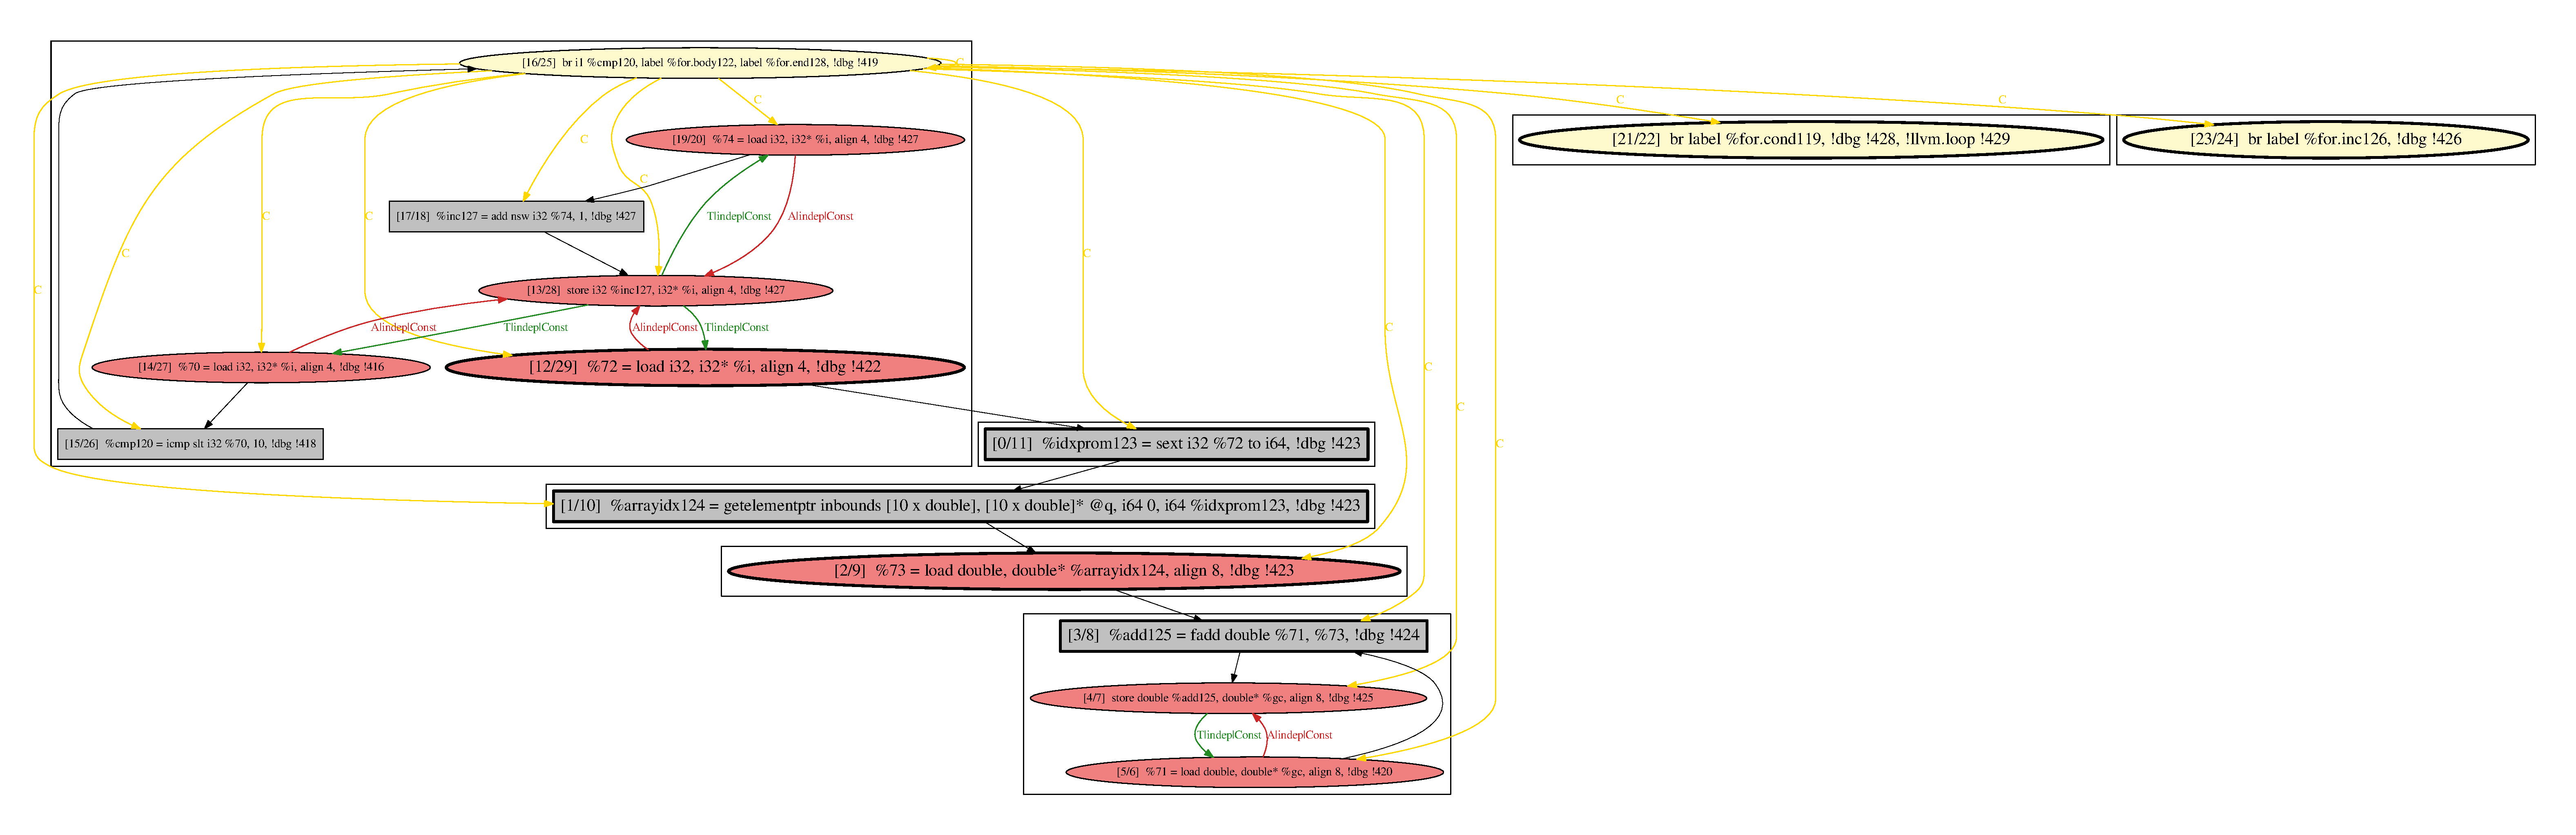
\includegraphics[width=\linewidth]{figs/metrics-example-loop-pdg.pdf}
	\caption{Program dependence graph (PDG) of the loop \ref{lst:metrics-loop-example}, as built and visualized by the PPar tool \ref{ppar-tool}.}
	\label{metrics-loop-example-pdg}
\end{figure}

\null\qquad Figure \ref{metrics-loop-example-pdg} above shows program dependence graph of the loop, given in the example. 


\subsection{Loop Proportion Metrics}
\label{metrics-loop-proportion-metrics}
\qquad The first group of metrics computes proportions of the loop. Like Halsted's software science metrics (see \ref{background-software-metrics-in-cs}), it draws an analogy with physical properties of objects (like size, volume, length, etc). This computation happens after PPar tool decouples a loop into iterator and payload code, as described in \ref{background-loop-decoupling}.  
\subsubsection{Loop Absolute Size}
\label{metrics-loop-absolute-size}
\qquad This metric represents the total amount of LLVM IR instructions in the loop. The intuition behind this metric is pretty staighforward: the bigger the loop, the harder it is to parallelize it. The metric has obvious drawbacks. The size of the loop does not, generally speaking, always correlates with loop parallelizability. However, it might be interesting to see, how loop absolute size correlates with loop parallelisability statistically. From figure \ref{metrics-loop-example-pdg} it is visible that the value of the metiric for the given loop \ref{lst:metrics-loop-example} is 15.
\subsubsection{Loop Payload Fraction}
\label{metrics-loop-payload-fraction}
\qquad This metric is complementary to loop absolute size metric and reflects the proportion in which iterator and payload divide the whole loop. There are different considerations behind this metric. For example, if the payload is too small relative to the size of the loop and does not perform significant amount of computations, then parallelization of this loop might not worth the effort.   

\subsubsection{Loop Proper SCCs number}
\label{metrics-loop-proper-sccs-number}
\qquad Once we decoupled a loop into iterator and payload parts, we can split payload part even further. Both iterator and payload are represented by subgraphs in the PDG of the loop. As was described in \ref{background-loop-decoupling}, iterator instructions form a strongly connected component (SCC), which has no incoming dependencies. Payload consists of a set of SCCs. These payload components have different sizes, starting from just 1 instruction and, principally, do not have any upper size limit. If SCC of PDG belongs to the payload of a loop and consists of more than 1 instruction, we call such SCC a \textbf{\textit{proper SCC}}. Usually, such components represent a true dependency in the body of a loop, preventing a loop from parallelization. Thus, the task of parallelizing compilers is to break the edges of such \textbf{\textit{proper (critical )}} SCCs, and transform these SCCs into smaller ones (possibly just 1 instruction). \newline
\null\qquad The example loop from the listing \ref{lst:metrics-loop-example} contains one such proper (critical) SCC. There is a cross-iteration dependency in the body of this loop. The partial sum is being accumulated in the \textit{gc} variable. We can see 2 edges (corresponding to true and anti dependencies) between variable \textit{gc} load and store instructions in the PDG shown on figure \ref{metrics-loop-example-pdg}. Despite the presense of cross-iteration dependency in the loop, Intel C/C++ compiler is capable of its parallelization with reduction techniques.\newline
\null\qquad Simplier loops, like the one shown on the listing \ref{lst:metrics-loop-example-1}, do not contain any SCCs of size greater than 1 (besides iterator SCC). Once we split such loops into iterator and payload parts, all SCCs in the payload are of 1 instruction size. Figure \ref{metrics-example-loop-1-pdg} provides illustration.
  
\begin{lstlisting}[float,floatplacement=H,caption={Parallelizible loop, with no cross-iteration dependencies. Taken from EP NAS benchmark.}, captionpos=b, label=lst:metrics-loop-example-1]
for (i = 0; i < 2 * NK; i++) {
	x[i] = -1.0e99;
}
\end{lstlisting}

\begin{figure}[htb]
	\centering
	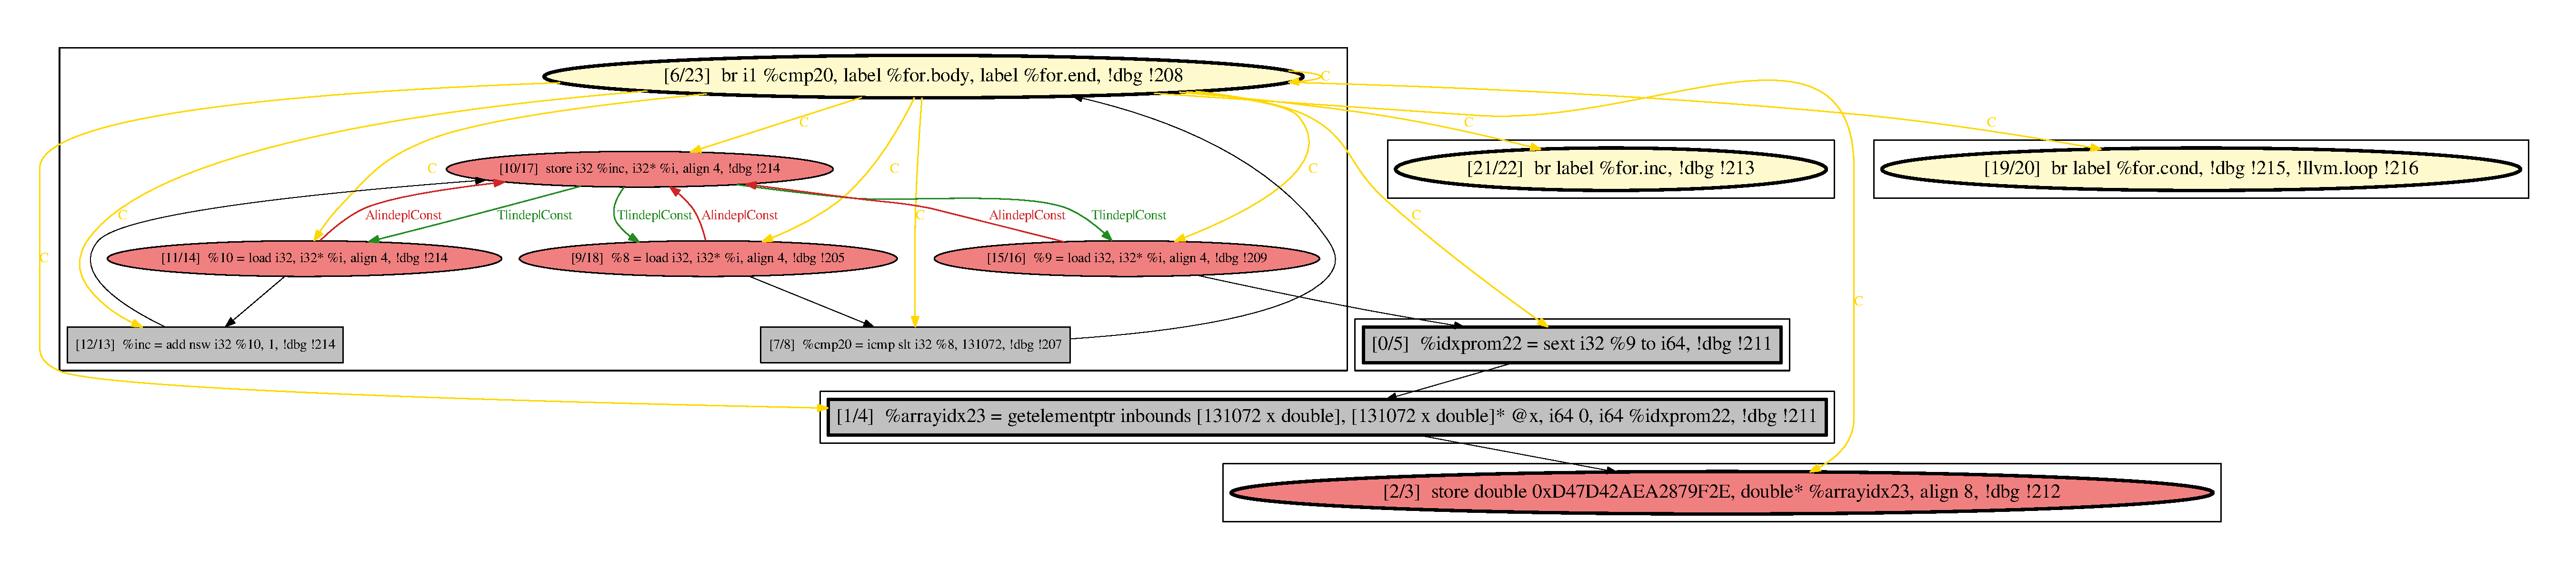
\includegraphics[width=\linewidth]{figs/metrics-example-loop-1-pdg.pdf}
	\caption{Program dependence graph (PDG) of the loop \ref{lst:metrics-loop-example-1}, as built and visualized by the PPar tool \ref{ppar-tool}.}
	\label{metrics-example-loop-1-pdg}
\end{figure}

\subsubsection{Loop Critical Payload Fraction}
\label{metrics-loop-critical-payload-fraction}
\qquad In the light of considerations given in the previous section, the fraction between critical and non-critical payload parts might have some correlation with loop parallelizability.  

\subsection{Loop Dependence Metrics}
\label{metrics-loop-dependence-metrics}

\subsection{Loop Cohesion Metrics}
\label{metrics-loop-cohesion-metrics}
\qquad As cohesion and coupling metrics have been proposed for computer software \ref{background-cohesion-and-coupling}, these properties can also be extended in context of this work. \newline
\null\qquad These properties characterize the degree of inter-dependence between different parts of loops. As was shown in the previous 

The main motivation behind the metrics out of this group is the tighter the parts of a loop are coupled together (in terms of dependencies), the harder it is going to be to split and parallalize the loop.   


